 \chapter{La détection d'objets}
\minitoc
\newpage
\pagestyle{fancy}
\fancyhead[L]{\chaptername \ \thechapter}
\fancyhead[R]{La détection d'objets}
\renewcommand{\headrulewidth}{1pt}
\fancyfoot[C]{\thepage}

\section{Introduction} 
La détection d'objet est un sous-domaine de vision par ordinateur dont le but de localiser la position de l'objet recherché et d'identifier en lui attribuant la classe appropriée dans une image numérique. Le besoin de détection d'objets est d'automatiser les tâches difficiles qui nécessitent une intervention humaine ou impossible à faire par l'homme. Par exemple, la tâche de lire le numéro d'immatriculation
de chaque voiture qui passe sur l'autoroute où les voitures passent à grande vitesse que l'œil humain avec le cerveau est incapable de percevoir quelques chiffres, sans parler du numéro d'enregistrement complet.

% =========== Objectif ===========
\section{Objectif}
L'objectif de la détection d'objets est divisé en 2 composants principaux; premièrement, la localisation d'objets et deuxièmement, l'identification ou la classification d'objets.
     \subsection{Localisation d'objet}
     Ce composant est la principale différence entre la détection d'objet dans l'image et la classification d'image où, dans la classification d'image, l'objet est identifié uniquement sans son emplacement dans l'image, d'autre part, dans la détection d'objet, l'objet est également localisé en utilisant la technique de la boîte englobante ou technique basée sur les pixels qui se divise également en segmentation sémantique et segmentation d'instance.
     \subsubsection{Boîte englobante (Bounding Box)}
     La technique de la boîte englobante est la méthode traditionnelle d'étiquetage des données dans l'image. Les cadres de délimitation sont des marqueurs d'annotation dessinés autour des objets dans une image. Contours mais en forme de forme rectangulaire. Il a fait l'objet des études les plus approfondies en raison de sa facilité d'utilisation et de calcul.

     \begin{figure}[H]
          \centering
          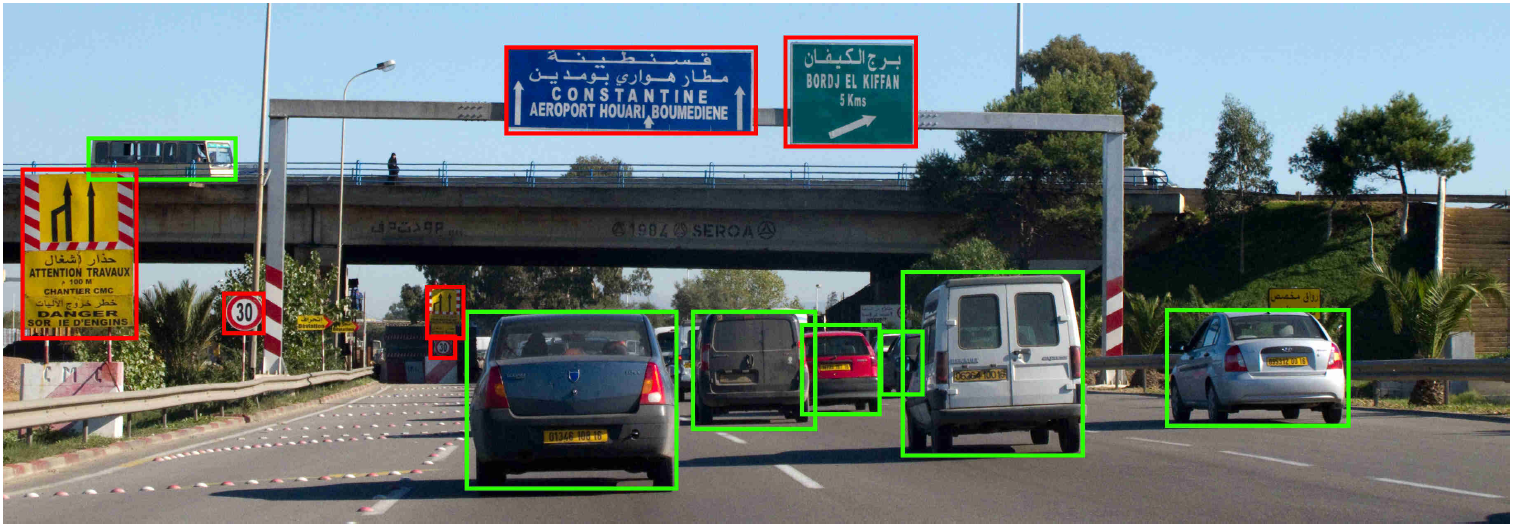
\includegraphics[height=5.7cm,width=16cm]{Chapitre1/im4.png}
          \caption{Exemple de détection basée sur la boîte englobante.}
          \label{im4}
          \end{figure}

     \subsubsection{Mask (niveau de pixel)}
     La deuxième technique utilisée dans la détection d'objets est basée sur les pixels. il nécessite de segmenter l'objet en pixel au lieu de la boîte englobante. cette technique donne un emplacement précis (au niveau du pixel) d'un objet et des pixels trouvés. les pixels produits peuvent aussi être appelés le masque. Il existe 2 types de segmentation, la premier est la segmentation sémantique où tous les objets de la même classe obtiennent le même pixel,
     \begin{figure}[H]
          \centering
          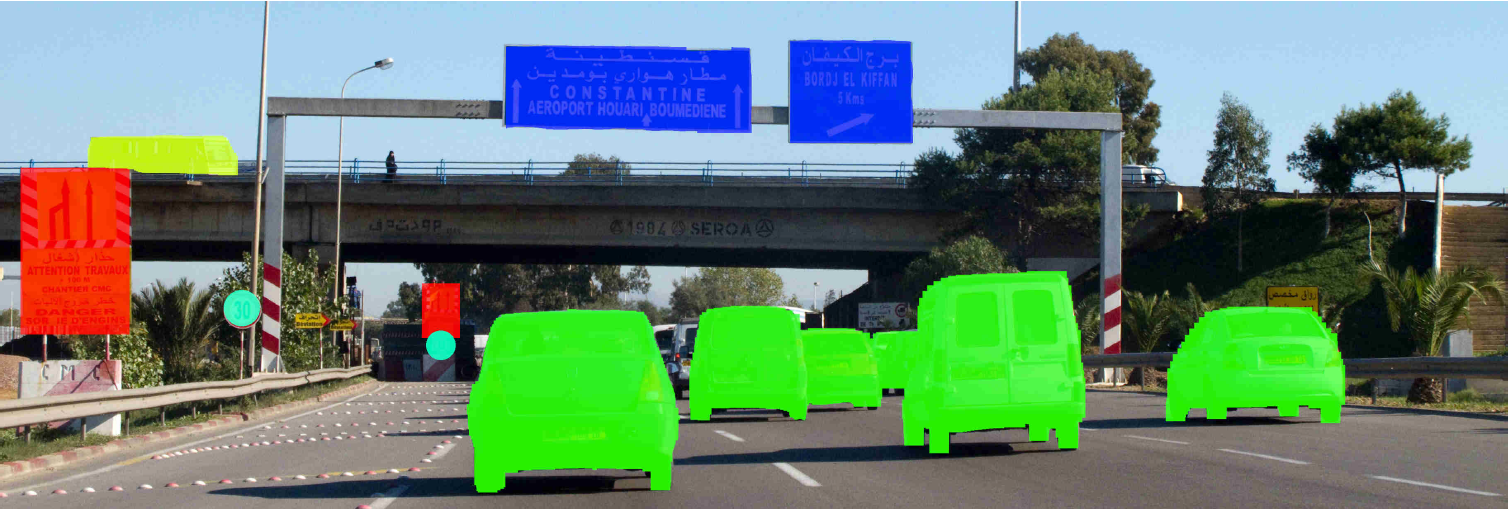
\includegraphics[height=5.7cm,width=16cm]{Chapitre1/im5.png}
          \caption{Exemple de détection de segmentation sémantique.}
          \label{im5}
          \end{figure}
     
          Où dans le deuxième type, la segmentation d'instance, chaque objet de l'image obtient son masque unique même s'il existe d'autres objets avec la même classe. En raison de la nature de bas niveau de cette technique, elle nécessite une puissance de calcul importante pour segmenter l'objet pixel par pixel, de plus cette technique est assez nouvelle et encore immature en raison des faibles études appliquées dans celle-ci.
     \begin{figure}[H]
          \centering
          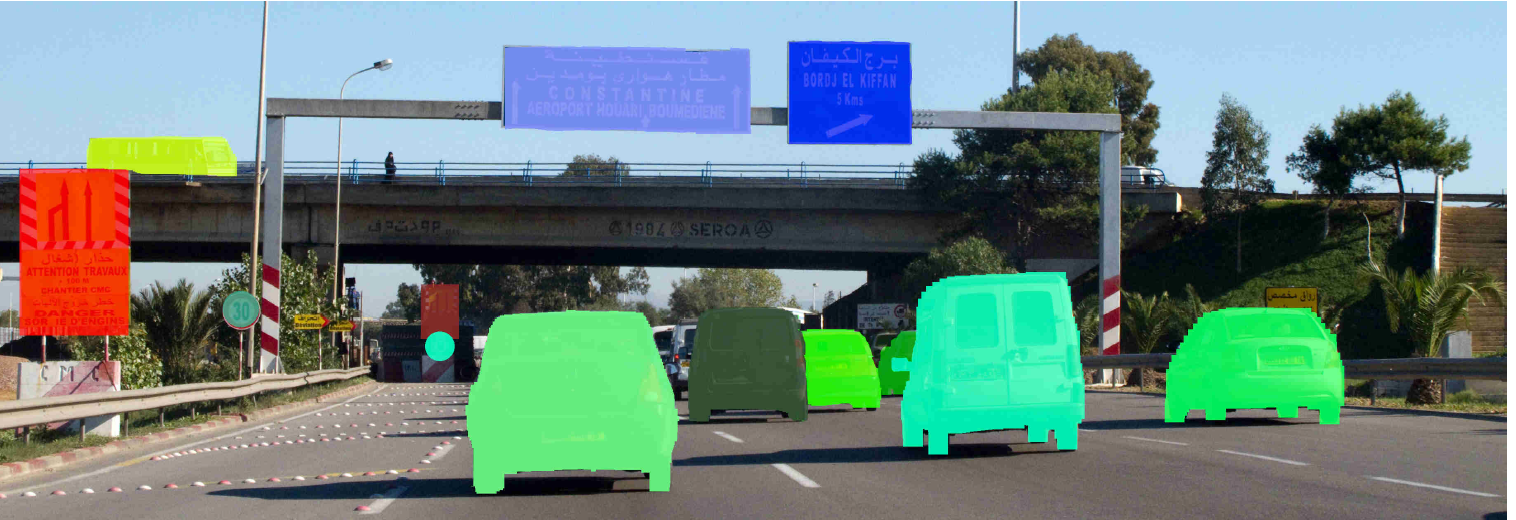
\includegraphics[height=5.7cm,width=16cm]{Chapitre1/im6.png}
          \caption{la segmentation d'instance.}
          \label{im6}
          \end{figure}


     \subsection{Classification d'objet}
     Le deuxième composant est la reconnaissance d'objets. La reconnaissance est la capacité du modèle (le réseau de neurones dans notre cas) à identifier un objet en fonction de certaines similitudes qu'il partage avec un autre objet que le modèle a déjà rencontré. La reconnaissance peut être basée sur une inférence ou une relation, c'est-à-dire une situation dans laquelle un modèle est capable de reconnaître un objet parce qu'il reconnaît les similitudes de forme et de propriétés.

     La reconnaissance peut également se produire parce que le modèle a rencontré l'objet exact lors d'une instance précédente Chez les êtres humains, la reconnaissance est un processus cognitif qui se déroule de manière transparente et presque instantanément sans délai. Le cerveau humain est capable d'apprendre et d'adapter des informations avec un minimum d'effort, de sorte que même les humains qui en sont encore aux stades de développement de leur existence peuvent facilement reconnaître les objets.

     Les humains peuvent reconnaître une multitude d'objets dans des images avec peu d'effort, même si l'image des objets peut varier quelque peu selon différents points de vue, dans de nombreuses tailles et échelles différentes ou même lorsqu'ils sont déplacés ou pivotés. Les objets peuvent même être reconnus lorsqu'ils sont partiellement masqués. La machine ou le modèle, cependant, ne possède pas de façon innée cette capacité cognitive.

     Pour que l'intelligence artificielle acquière ce niveau de compétence, elle doit acquérir une formation. Cette formation est généralement acquise en apprenant les jeux de données du modèle. Cette tâche reste un défi pour les systèmes de vision par ordinateur étant donné que ces modèles doivent être entraînés pour chaque classe d'objets qu'ils sont censés reconnaître.

     \begin{figure}[H]
          \centering
          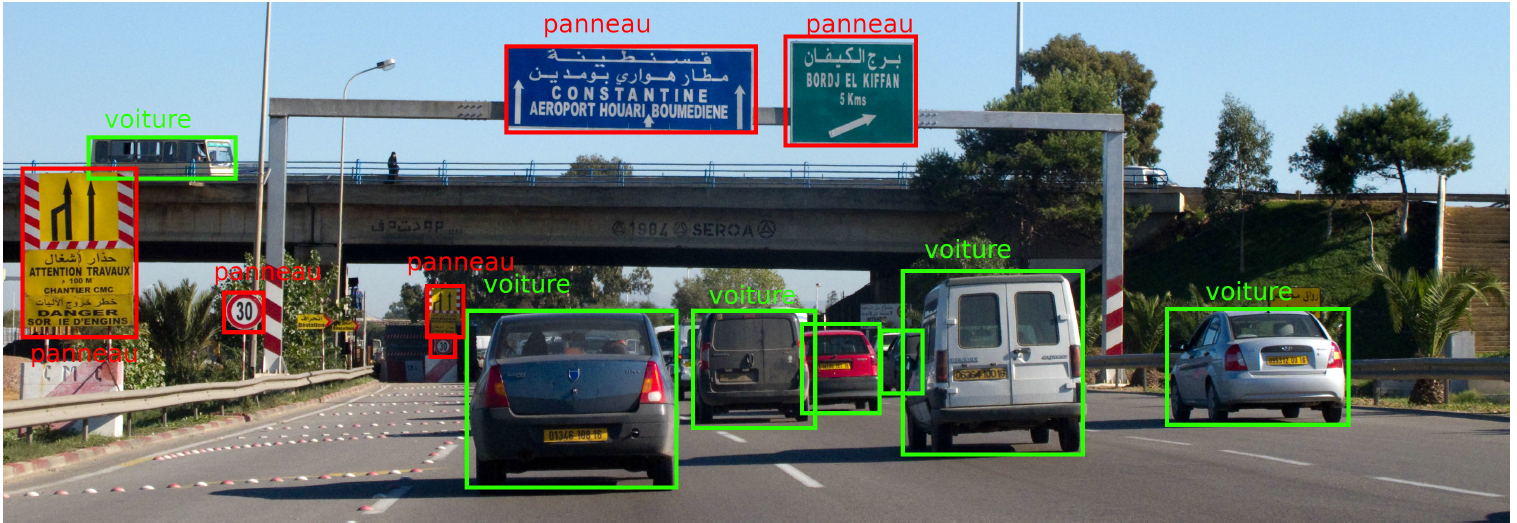
\includegraphics[height=6cm,width=16cm]{Chapitre1/im7.png}
          \caption{Détection d'objet basée sur la boîte englobante avec le nom de la classe.}
          \label{im7}
          \end{figure}

\section{Historique}
L'histoire de la détection d'objets est divisée en 2 époques la première époque est nommée l'époque traditionnelle ou l'époque avant l'apprentissage profond où les ressources étaient extrêmement limitées qui incluent la faible puissance de calcul des machines avec le manque de représentation d'image efficace, par conséquent, les algorithmes qui ont été construits à cette époque sont basés sur des caractéristiques sélectionnées manuellement, comme les détecteurs Viola Jones développé par Paul Viola and Michael Jones en 2001
qui permis la détection de visages humains en temps réel à l'aide d'une fenêtre coulissante qui recherche les caractéristiques du visage, malheureusement, la détection d'objets a atteint un plateau après 2010, car les performances des caractéristiques sélectionnées manuellement sont devenues saturées.

Après la généralisation d'Internet dans le monde entier et l'augmentation des données flottant sur le Web qui ont conduit à la création d'ImageNet, une grande base de données visuelle conçue pour être utilisée dans la recherche de logiciels de reconnaissance visuelle d'objets. et l'augmentation drastique de la puissance de calcul des machines provoquée par le développement de systèmes de calcul parallèles comme les super-machines de calcul haute performance (HPC), A ouvert la voie à l'apprentissage profond en particulier aux réseaux de neurones convolutifs (CNN) A ouvert la voie à l'apprentissage en profondeur, en particulier aux réseaux de neurones
convolutifs et le plus célèbre est AlexNet implementé par Alex Krizhevsky en 2012. De nombreux algorithmes sont apparus après pour amélioré les performances et le résultat et nous utiliserons l'algorithme YOLO plus tard.

%\section{Etat de l'art des techniques de détection d'objets}

----

% =========== Apps ===========
\section{Les applications de la détection d'objets}
La détection d'objets fait son entrée dans un large éventail d'industries, avec des cas d'utilisation allant de la sécurité personnelle à la productivité sur le lieu de travail. La détection et la reconnaissance d'objets sont appliquées dans de nombreux domaines de la vision par ordinateur, notamment la récupération d'images, la sécurité, la surveillance, les systèmes de véhicules automatisés et l'inspection des machines. Des défis importants subsistent dans le domaine de la reconnaissance d'objets. Les possibilités sont infinies en ce qui concerne les futurs cas d'utilisation de la détection d'objets. Dans cette section, nous discutons  certaines applications actuelles et futures  des systèmes de détection d'objets dans divers domaines..
     % =========== OCR ===========
     \subsection{Reconnaissance optique de caractères (OCR)}
     La reconnaissance optique de caractères (OCR) est le processus qui convertit une image de texte en un format de texte lisible par machine.

     La plupart des workflows d'entreprise impliquent la réception d'informations de la presse écrite. Les formulaires papier, les factures, les documents juridiques numérisés et les contrats imprimés font tous partie des processus commerciaux. Ces gros volumes de paperasse prennent beaucoup de temps et d'espace à stocker et à gérer. Bien que la gestion des documents sans papier soit la voie à suivre, la numérisation du document en une image pose des défis. Le processus nécessite une intervention manuelle et peut être fastidieux et lent.

     De plus, la numérisation du contenu de ce document crée des fichiers image avec le texte caché à l'intérieur. Le texte des images ne peut pas être traité par un logiciel de traitement de texte de la même manière que les documents texte. La technologie OCR résout le problème en convertissant les images textuelles en données textuelles pouvant être analysées par d'autres logiciels d'entreprise. Vous pouvez ensuite utiliser les données pour effectuer des analyses, rationaliser les opérations, automatiser les processus et améliorer la productivité.
     \begin{figure}[H]
          \centering
          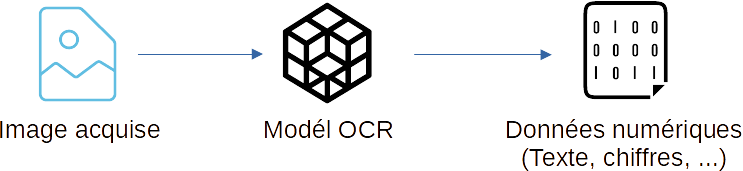
\includegraphics[height=4cm,width=16cm]{Chapitre1/img11.png}
          \caption{Reconnaissance optique de caractères (OCR).}
          \label{img11}
          \end{figure}
     
     % =========== Self-Driving ===========
     \subsection{Voitures autonomes}
     Une voiture autonome est un véhicule capable de détecter son environnement et de fonctionner sans intervention humaine. Un passager humain n'est pas tenu de prendre le contrôle du véhicule à tout moment, et un passager humain n'est pas du tout tenu d'être présent dans le véhicule. Une voiture autonome peut aller partout où va une voiture traditionnelle et faire tout ce qu'un conducteur humain expérimenté fait.

     Les voitures autonomes créent et maintiennent une carte de leur environnement basée sur une variété de capteurs situés dans différentes parties du véhicule. Des capteurs radar surveillent la position des véhicules à proximité. Des caméras vidéo qui prennent des images de son environnement, là où la détection d'objets joue un rôle essentiel pour détecter les feux de circulation, lire les panneaux de signalisation, suivre les autres véhicules et rechercher les piétons qui seront utilisés par la voiture autonome pour prendre une décision.
     \begin{figure}[H]
          \centering
          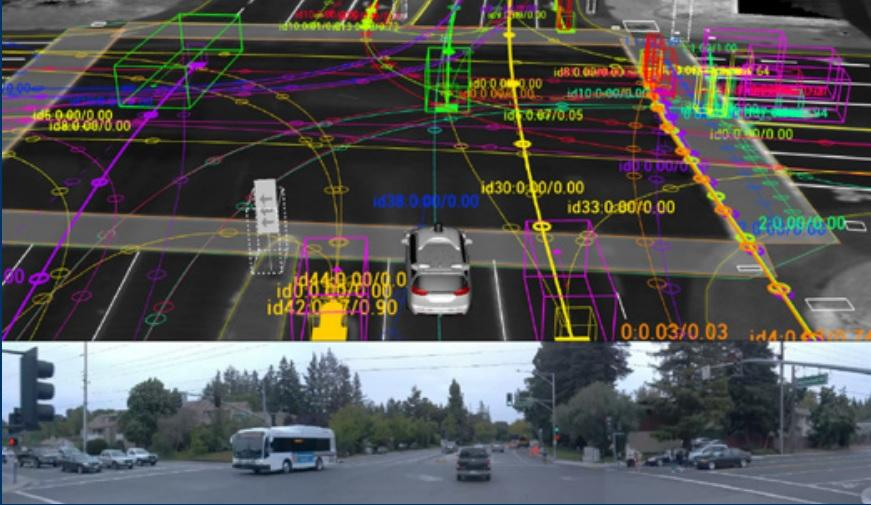
\includegraphics[height=7cm,width=12cm]{Chapitre1/img12.jpg}
          \caption{carte de l'environnement des voitures autonomes générée à l'aide de la détection d'objets.}
          \label{img12}
          \end{figure}
     
     % =========== Biometrics ===========
     \subsection{Biométrie}
     La biométrie est la mesure et l'analyse statistique des caractéristiques physiques et comportementales uniques des personnes. La technologie est principalement utilisée pour l'identification et le contrôle d'accès ou pour l'identification de personnes.
     
     L'authentification par vérification biométrique est de plus en plus courante dans les systèmes de sécurité d'entreprise et publics, l'électronique grand public et les applications de point de vente. En plus de la sécurité, le moteur de la vérification biométrique a été la commodité, car il n'y a pas de mots de passe à retenir ni de jetons de sécurité à transporter. Certaines méthodes biométriques, telles que la reconnaissance faciale et la reconnaissance de l'iris, sont fortement basées sur la détection d'objets.
     \begin{figure}[H]
          \centering
          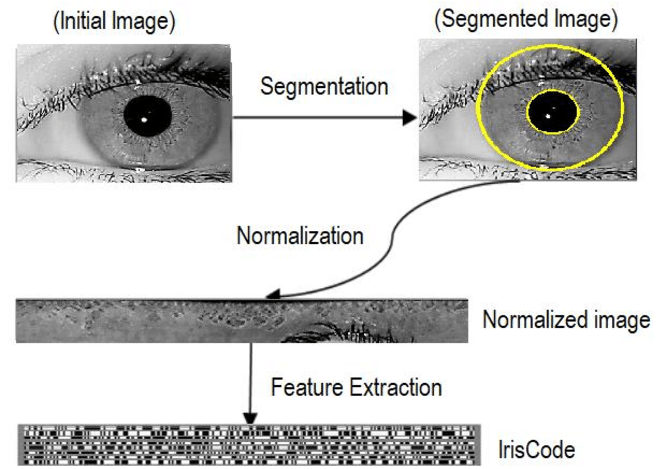
\includegraphics[height=7cm,width=12cm]{Chapitre1/img13.png}
          \caption{Identification de l'iris à l'aide de la détection d'objet.}
          \label{img13}
          \end{figure}
     
     % =========== Acitivity ===========
     \subsection{Reconnaissance d'activités}
     La reconnaissance d'activité vise à reconnaître les actions et objectifs d'un ou plusieurs agents à partir d'une série d'observations sur les actions des agents et les conditions environnementales. Ce domaine de recherche a attiré l'attention de plusieurs communautés informatiques en raison de sa capacité à fournir un support personnalisé pour de nombreuses applications différentes et de sa connexion à de nombreux domaines d'études différents tels que l'interaction homme-machine ou la sociologie.
     \begin{figure}[H]
          \centering
          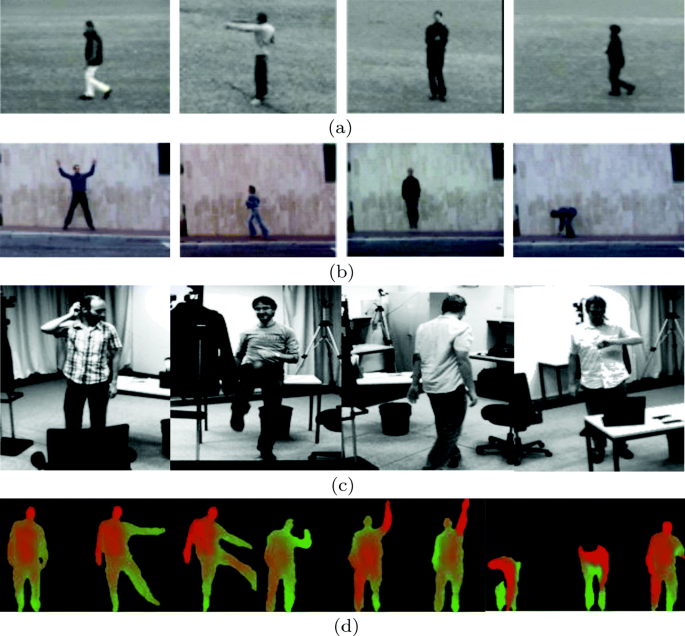
\includegraphics[height=10cm,width=12cm]{Chapitre1/img14.png}
          \caption{Reconnaissance d'activités.}
          \label{img14}
          \end{figure}

     % =========== Med ===========
     \subsection{Imagerie médicale}
     Les outils de traitement d'images médicales jouent un rôle de plus en plus important pour aider les cliniciens dans le diagnostic, la planification de la thérapie et les interventions guidées par l'image. Le suivi précis, robuste et rapide d'objets anatomiques déformables tels que le cœur est une tâche cruciale dans l'analyse d'images médicales.
     \begin{figure}[H]
          \centering
          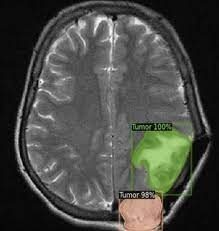
\includegraphics[height=7cm,width=7cm]{Chapitre1/img15.jpg}
          \caption{Détection de tumeurs cérébrales à l'aide de méthodes de détection d'objets.}
          \label{img15}
          \end{figure}

     % =========== Robo ===========
     \subsection{Robotique}
     Les robots d'assistance autonomes doivent être dotés de la capacité de traiter les données visuelles en temps réel afin qu'ils puissent réagir de manière adéquate pour s'adapter rapidement aux changements de l'environnement. La détection et la reconnaissance fiables d'objets sont généralement une première étape nécessaire pour atteindre cet objectif.
     \begin{figure}[H]
          \centering
          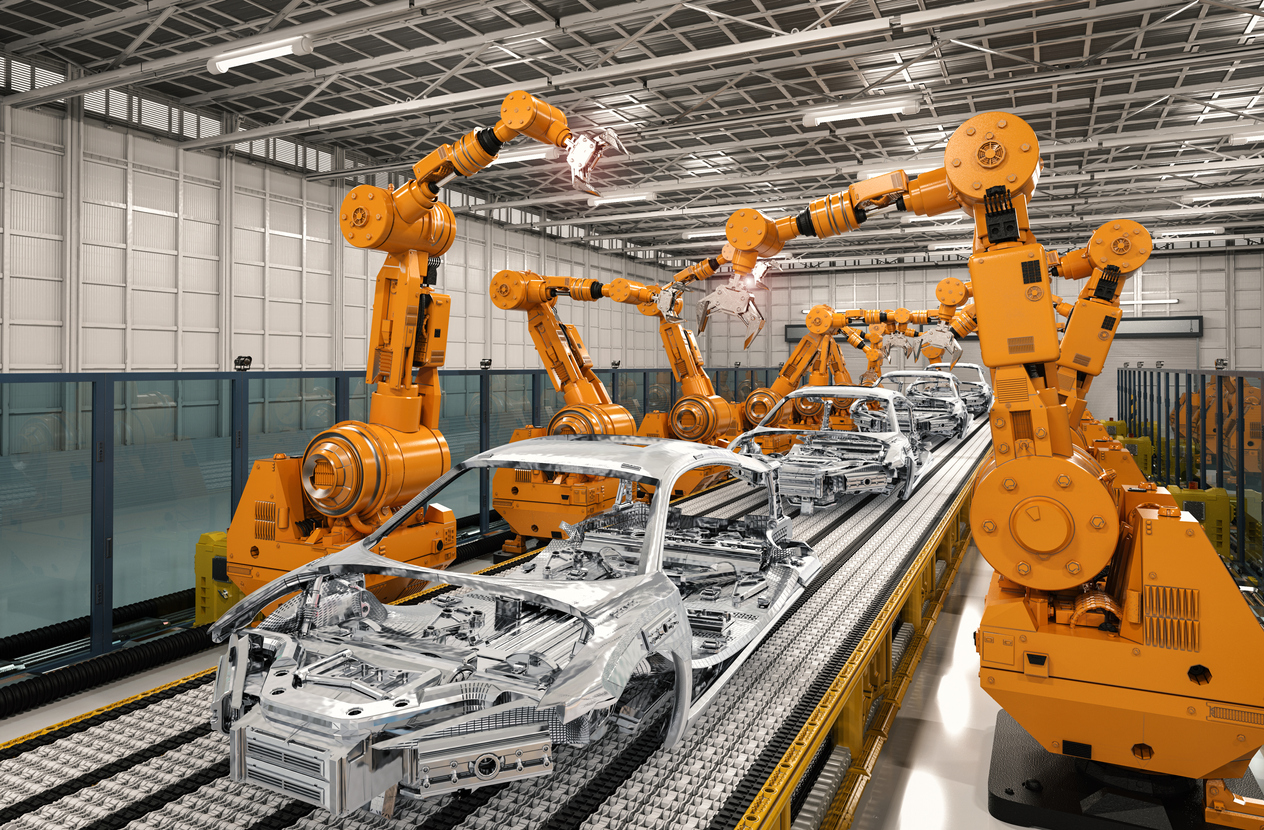
\includegraphics[height=7cm,width=12cm]{Chapitre1/img16.jpg}
          \caption{Mains robotiques utilisées dans la construction automobile.}
          \label{img16}
          \end{figure}
     
     % =========== Factory ===========
     \subsection{Production industrielle}
     Les usines du monde entier s'efforcent de produire des produits de la
     meilleure qualité avec un coût de production minimum. Cependant, pour
     atteindre cet objectif, les usines doivent embaucher de la main-d'œuvre pour vérifier la qualité des composants, ce qui augmente le coût de production et d'autres problèmes liés au travail manuel. comme la dextérité et la productivité du travailleur. La détection d'objets résout les problèmes liés au travail manuel. il garantit que les bons composants sont utilisés dans les chaînes de montage et que les processus corrects sont suivis avec une précision et une exactitude élevées, plus qu'un travailleur manuel et à moindre coût.
     \begin{figure}[H]
          \centering
          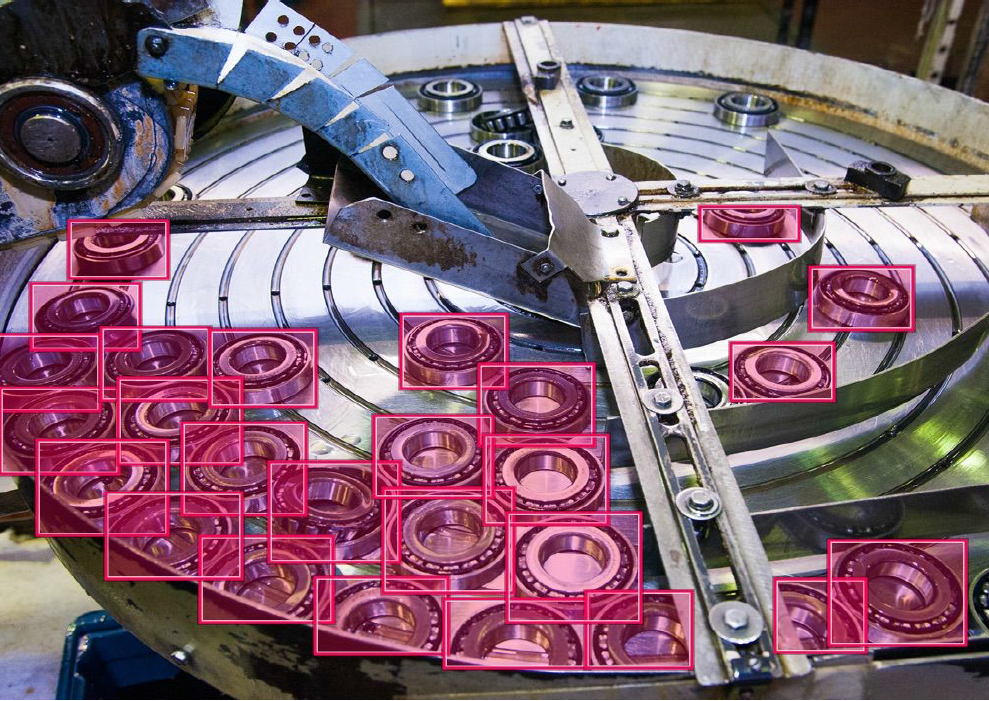
\includegraphics[height=7cm,width=12cm]{Chapitre1/im8.png}
          \caption{Détection d'objets utilisée pour détecter les pièces fabriquées mal formées.}
          \label{im8}
          \end{figure}
     
     
     % =========== Security ===========
     \subsection{Surveillance et sécurité}
     Dans les grandes villes où la population est très élevée, dans les zones industrielles, les grandes banques et de nombreuses autres zones hautement sensibles, la sécurité est indispensable 24 heures sur 24 et il est presque impossible pour un être humain d'atteindre ce niveau. La détection d'objets est donc une solution à ce type de problèmes où elle suit les mouvements des visiteurs, suit les comportements des individus ou des véhicules, fait la distinction entre les activités autorisées et non autorisées et signale lorsqu'un objet inattendu nécessite une enquête. tout cela 24 heures sur 24 sans arrêt et aussi à moindre coût de maintenance.
     \begin{figure}[H]
          \centering
          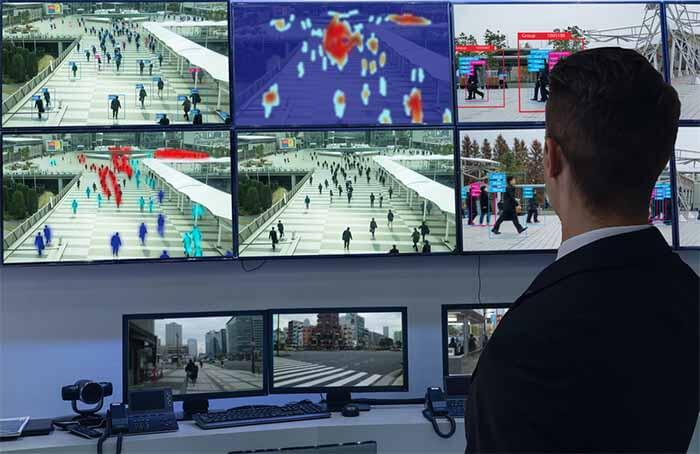
\includegraphics[height=6cm,width=12cm]{Chapitre1/img17.jpeg}
          \caption{Détection d'objets utilisée dans la sécurité et la surveillance.}
          \label{im17}
          \end{figure}

     % =========== Recherche visuelle ===========
     \subsection{Recherche visuelle}   
     Puisqu'une image peut contenir des dizaines d'objets, la détection d'objets rend aussi simple que possible le démarrage d'une expérience de découverte à partir de n'importe lequel d'entre eux. De la même manière que la saisie semi-automatique améliore l'expérience de recherche de texte, la détection d'objets fait de la recherche visuelle une expérience plus fluide. La détection d'objets dans la recherche visuelle permet également de nouvelles fonctionnalités, telles que la correspondance d'objet à objet.
     \begin{figure}[H]
          \centering
          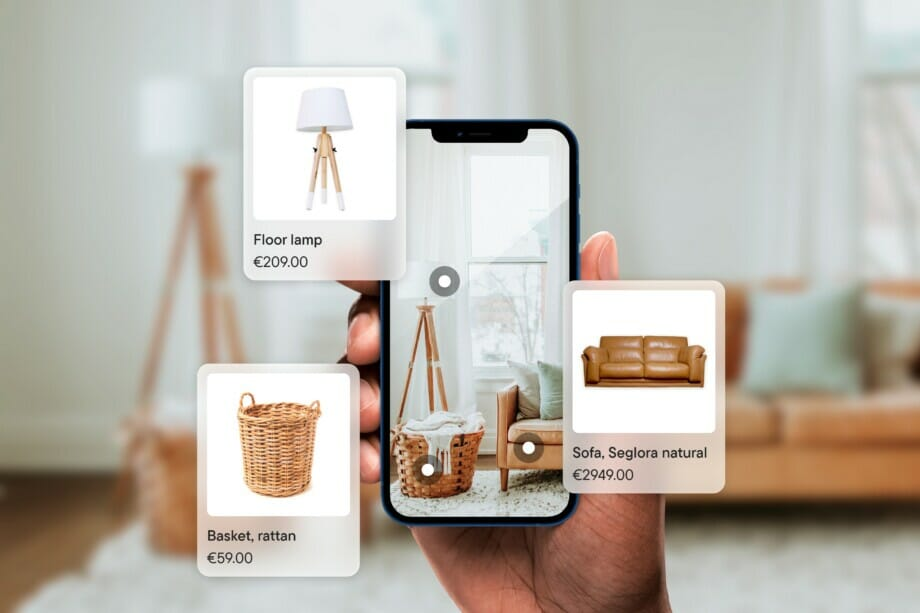
\includegraphics[height=8cm,width=14cm]{Chapitre1/img18.jpg}
          \caption{Shopping intelligent grâce à la détection d'objets.}
          \label{im18}
          \end{figure}

\section{Conclusion}
La détection d'objets fait son entrée dans un large éventail d'industries, avec des cas d'utilisation allant de la sécurité personnelle à la productivité sur le lieu de travail. La détection et la reconnaissance d'objets sont appliquées dans de nombreux domaines de la vision par ordinateur, notamment la récupération d'images, la sécurité, la surveillance, les systèmes de véhicules automatisés et l'inspection des machines. Des défis importants subsistent dans le domaine de la reconnaissance d'objets. Les possibilités sont infinies en ce qui concerne les futurs cas d'utilisation de la détection d'objets.

